\chapter{Navigation dans les briques}

% 2 Etapes et briques
% 2.1 Vue globale
% 2.2 Ouverture d'une brique
% 2.3 Edition des relations

Une fois la session créée, l'utilisateur peut accéder à l'ensemble des briques qui font intervenir les acteurs qu'il a sélectionnés.\\

Les différentes briques sont regroupées par étape. Les étapes correspondent aux différentes phases du cas étudié.\\

\section{Vues globales}

Lors de l'ouverture ou de la création d'une session, une interface présentant les différentes vues globales apparaît. Chaque vue globale présente les briques d'une étape (il y a une vue globale par étape qui contient au moins une brique). L'arborescence sur la gauche de la fenêtre présente un dossier par étape, chacun d'eux contenant les briques de l'étape et les exports de ces briques (voir partie \ref{export}).\\

Pour accéder à la vue globale, il suffit de cliquer sur son onglet ("Vue globale"). 

\begin{figure}[h!]
\centering

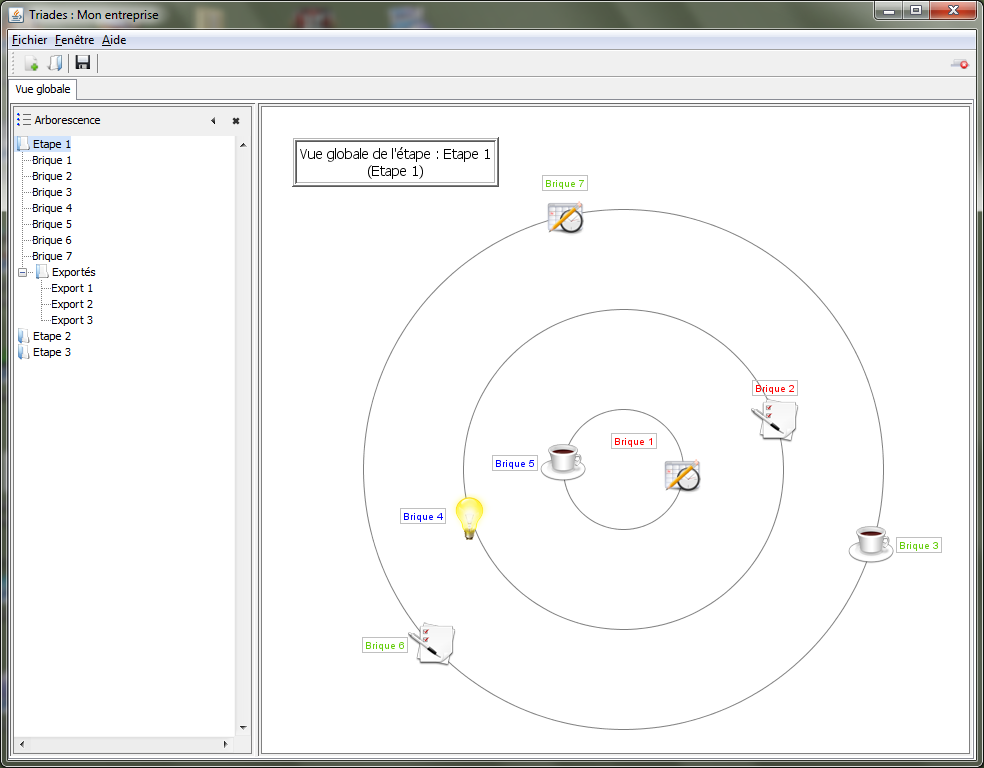
\includegraphics[scale=0.35]{images/vue_globale.png}
\caption{Vue globale d'une étape}

\end{figure}

Chaque vue globale se présente sous la forme de 3 cercles concentriques. Les briques sont disposées en fonction de l'importance des acteurs sélectionnés par l'utilisateur dans ces briques.
\begin{itemize}
\item Dans les briques les plus au centre, les acteurs principaux de l'utilisateur ont un rôle central.
\item Dans le deuxième cercle, les acteurs principaux ont un rôle secondaire et/ou les acteurs secondaires ont un rôle central ou secondaire.
\item Dans le troisième cercle les acteurs sélectionnés ont un rôle peu important.\\
\end{itemize}

La couleur des étiquettes des différentes briques indique si les relations de ces briques ont été remplies ou non, et si elles sont en écart. 
\begin{itemize}
\item Le bleu correspond à une brique où des relations n'ont pas été remplies.
\item Le rouge correspond à une brique où au moins une des relations est en écart.
\item Le vert correspond à une brique où toutes les relations sont remplies et aucune ne présente d'écart.
\end{itemize}

Le rouge étant prioritaire sur le bleu, une brique comportant des relations pas encore remplies et au moins une relation en écart apparaîtra en rouge.\\

Il est possible d'accéder d'accéder à toutes les exportations réalisée sur une brique en faisant un clic droit sur cette dernière (voir le chapitre \ref{export} sur les exportations).\\

Pour ouvrir une brique, il suffit de faire un double-clic sur son icône dans une vue globale ou sur la ligne de l'arbre correspondante. Un nouvel onglet apparaĩt  pour afficher cette brique. Plusieurs briques peuvent être ouverte en même temps. 

\section{Briques et relations}
Chaque brique représente une situation qu'il est possible de rencontrer dans la réalité. Les différents éléments du schéma correspondent aux acteurs, aux moyens et à l'activité qui composent la brique.\\

\begin{figure}[h!]
\centering
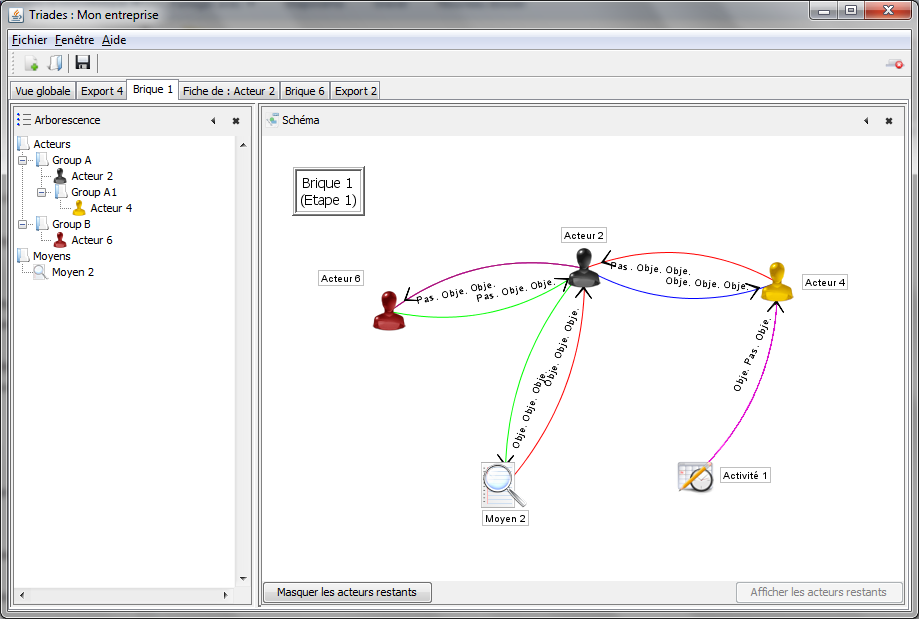
\includegraphics[scale=0.55]{images/brique.png}
\caption{Vue globale d'une étape}

\label{brique}
\end{figure}

Les éléments apparaissent progressivement afin de permettre à l'utilisateur d'assimiler les différents éléments de la situation. Les deux boutons situés en dessous du schéma permettent d'afficher et de masquer les éléments de la brique.\\

Les éléments apparaissent dans l'ordre suivant :\\
\begin{enumerate}
\item Les moyens, les activités, les acteurs principaux et ceux ayant un rôle central dans la brique.
\item Les acteurs secondaires et ceux ayant un rôle secondaire.
\item Les acteurs restants.\\
\end{enumerate}

Les relations entre deux acteurs sont représentées par des flèches entre deux éléments d'un schéma. Ces flèche sont orientées, ainsi une flèche allant d'un acteur A vers un acteur B représente la relation que A a envers B, la relation retour (ie. de B vers A) est associée à la flèche retour.\\

Deux manières permettent de sélectionner une arête. Soit en cliquant dessus (ou sur son étiquette), soit en faisant un clic continu à partir du premier acteur jusqu'au deuxième.\\

\begin{figure}[h!]
\centering
\Ovalbox{
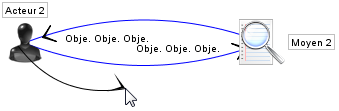
\includegraphics[height=25pt]{images/selection_1.png}
}
\Ovalbox{
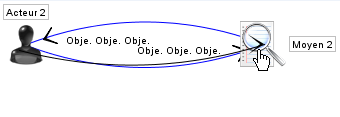
\includegraphics[height=25pt]{images/selection_2.png}
}
\Ovalbox{
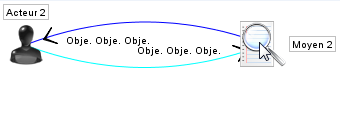
\includegraphics[height=25pt]{images/selection_3.png}
}
\caption{La sélection d'une arête à l'aide d'un clic continu.}

\end{figure}

Lorsqu'on sélectionne une relation, une fenêtre apparaît. Elle permet de consulter et modifier la relation. Il est possible de définir les objectifs et les moyens réels de chaque temps d'action. Une liste de possibilité est fournie pour chaque champ. La relation structurelle est affichée dans cette fenêtre mais ne peut pas être modifiée.\\

La petite flèche située sur la gauche d'un objectif permet de répliquer l'objectif et le moyen réel au temps d'action suivant.

\begin{figure}[h!]
\centering
\Ovalbox{
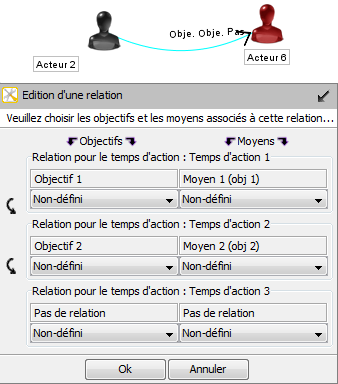
\includegraphics[scale=0.75]{images/edition_relation.png}
}
\caption{Pop-up d'édition d'une relation}
\label{edition_relation}
\end{figure}

Les relations apparaissent d'une couleur différente en fonction de leur état. Le code couleur utilisé est le même que celui des briques (voir figure~\ref{brique} pour les couleurs des arêtes) :
\begin{itemize}
\item Bleu pour une relation incomplète (certains objectifs sont encore à "Non-défini").
\item Violet pour une relation en écart au niveau d'un moyen (un des moyens réels est différents du moyen structurel mais les objectifs sont tous en accords).
\item Rouge pour une relation en écart au niveau d'un objectif (un des objectifs réels est en écart, le moyen n'est pas pris en compte).
\item Vert pour une relation réelle en accord avec la relation structurelle (tous les objectifs et les moyens concordent).
\end{itemize}

Attention, n'oubliez pas de faire apparaître l'ensemble des acteurs pour avoir accès à toutes les relations d'une brique.\\

Les relations sont associées à des info-bulles qui fournissent un résumé complet des objectifs et des moyens de la relation. Il suffit de placer la souris sur une flèche pendant une seconde pour faire apparaître l'info-bulle.\\

Il est possible d'ajouter une relation absente. Cependant, tous les objectifs structurels seront mis à "Pas de relation", de ce fait cette relation sera forcément en écart. Si l'utilisateur définit tous les objectifs réels à "Pas de relation", l'arête ne sera pas affichée.\\

L'arborescence sur la gauche de la fenêtre présente l'ensemble des acteurs présents dans la brique. Elle permet de sélectionner rapidement un acteur et aussi d'accéder à sa fiche à l'aide d'un clic droit.\\

Il est possible de déplacer un sommet en maintenant la touche "Shift" (majuscule) appuyée tout en cliquant sur le sommet. De même pour déplacer l'ensemble des sommets, il faut cliquer sur la touche "Ctrl" tout en cliquant.\\ 

\section{Etiquettes par défaut des arêtes}
Il est possible de changer le contenu par défaut des étiquettes des arêtes dans les briques. Le sous-menu "Etiquettes des arêtes des briques" dans le menu Edition offre les possibilités suivantes :\\
\begin{itemize}
\item \textbf{Relations structurelles} : Affiche les 4 premiers caractères des relations structurelles de chaque temps d'action.\\
\item \textbf{Relations réelles} : De même avec les relations réelles.\\
\item \textbf{Relation au temps d'action : *} : Affiche la relation structurelle et la relations réelle pour le temps d'action sélectionné.\\ 
\end{itemize}

Cette option ne concerne que les relations dans les briques. Dans les exports, ces étiquettes sont contrôlées par les options globales de l'export (voir paragraphe \ref{globalExport}).\\

\begin{figure}[h!]
\centering
\Ovalbox{
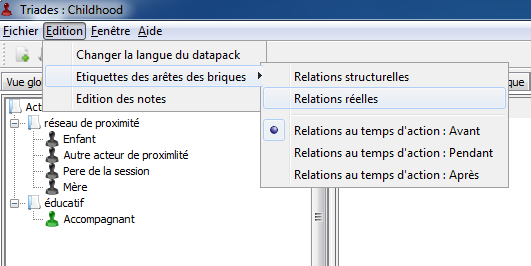
\includegraphics[width=0.5\textwidth]{images/menu_edition.png}
}
\caption{Le menu de choix du contenu par défaut\\des étiquettes des arêtes}
\label{menu_edition}
\end{figure}


\section{Edition des notes dans les briques}
Chaque brique est associée à une note. Cela permet d'ajouter des informations pour décrire une situation. Par défaut, les notes ne sont pas éditables. Il faut activer l'option "Edition des notes" dans le menu édition avant de pouvoir les modifier (voir image \ref{menu_edition}).\\

Les notes sont accessibles à l'aide du cadre présent en haut à droite de la zone d'affichage d'une brique. Attention, une note n'est accessible que dans la brique de la session où elle a été éditée. Elle ne sera pas accessible dans les autres sessions.\\

\begin{figure}[h!]
\centering
\begin{subfigure}{\textwidth}

\centering
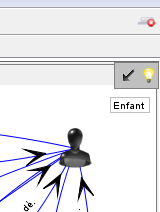
\includegraphics[width=0.4\textwidth]{images/note_fermee.png}
\caption{Une note lorsqu'elle n'est pas affichée}
\end{subfigure}
\begin{subfigure}{\textwidth}

\centering
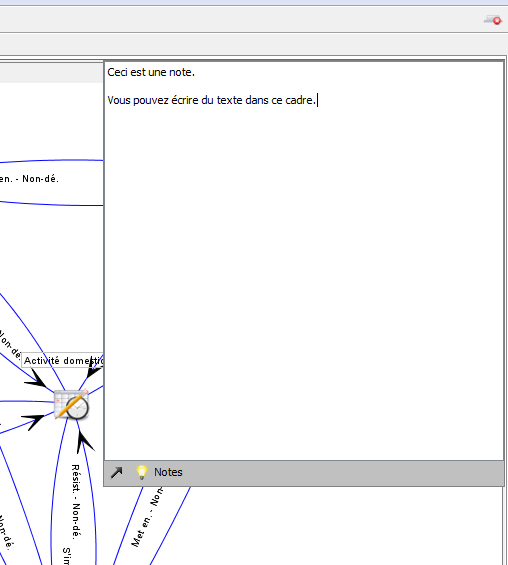
\includegraphics[width=0.4\textwidth]{images/note_ouverte_edition.png}
\caption{Une note ouverte en cours d'édition}
\end{subfigure}
\begin{subfigure}{\textwidth}

\centering
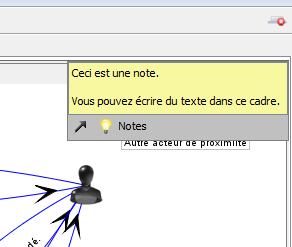
\includegraphics[width=0.4\textwidth]{images/note_ouverte_pas_edition.png}
\caption{Une note en mode affichage uniquement}
\end{subfigure}
\caption{Différents états d'une note}
\end{figure}

